
\section{Architecture Integration}

\subsection{Model Support}

\begin{table}[H]
\centering
\small
\begin{tabular}{llll}
\toprule
\textbf{Model} & \textbf{$N$ tested} & \textbf{Nystr m path} & \textbf{Fallback} \\
\midrule
DistilBERT & 128 &  & Dense \\
RoBERTa & 128 &  & Dense \\
GPT-2 & 128 & (causal) & Dense causal \\
Qwen3.5 & 128 & (causal) & Dense causal \\
\bottomrule
\end{tabular}
\end{table}

\textbf{Note.} At $N = 128$, all four models use the \textbf{dense fallback}. The 
Nystr m branch only activates for $N > 128$.

\subsection{DistilBERT (Flat)}

\begin{lstlisting}
distilbert.transformer.layer.0.attention
+-- q\_lin
+-- k\_lin
+-- v\_lin
+-- out\_lin
\end{lstlisting}

\textbf{Extraction:}
\begin{lstlisting}
w\_q = src.q\_lin.weight.data
w\_k = src.k\_lin.weight.data
w\_v = src.v\_lin.weight.data
w\_o = src.out\_lin.weight.data
\end{lstlisting}

\texttt{is\_nested\_encoder = False}.

\subsection{RoBERTa (Nested)}

\begin{lstlisting}
roberta.encoder.layer.0.attention
+-- self
|   +-- query, key, value
+-- output
    +-- dense
\end{lstlisting}

\textbf{Nested detection:}
\begin{lstlisting}
if hasattr(src, "self") and hasattr(src, "output"):
    is\_nested = True
\end{lstlisting}

\texttt{is\_nested\_encoder = True}. The outer \texttt{output.dense} applies projection.

\subsection{GPT-2 (Causal Conv1D)}

\begin{lstlisting}
transformer.h.0.attn
+-- c\_attn  (Conv1D)
+-- c\_proj  (Conv1D)
\end{lstlisting}

\textbf{Split c\_attn:}
\begin{lstlisting}
c\_w = src.c\_attn.weight.data
if "Conv1D" in type(src.c\_attn).\_\_name\_\_ or c\_w.shape[0] \textless{} c\_w.shape[1]:
    c\_w = c\_w.t()
q\_w, k\_w, v\_w = c\_w.chunk(3, dim=0)
\end{lstlisting}

\textbf{Causal decoder detection:} \texttt{self.is\_decoder = True} $\to$ dense causal 
attention.

\subsection{Qwen3.5 (GQA + RoPE)}

\begin{lstlisting}
model.layers.0.self\_attn
+-- q\_proj
+-- k\_proj
+-- v\_proj
+-- o\_proj
\end{lstlisting}

\textbf{GQA:} \texttt{repeat\_kv} during forward.

\textbf{RoPE:} applied after projection via \texttt{position\_embeddings}.

\textbf{Causal decoder detection:} \texttt{self.is\_decoder = True}.

\subsection{Nested Encoder Bypass}

\begin{lstlisting}
context = torch.matmul(attn\_weights, V)
context = context.transpose(1, 2).contiguous().view(...)

if self.is\_nested\_encoder:
    return context, None    # Skip out\_proj
else:
    return self.out\_proj(context), None
\end{lstlisting}

\subsection{Injection Hook}

\begin{lstlisting}
def inject\_nystrom(layer, model\_config, comp\_config, old\_attn=None, **kwargs):
    src\_attn = old\_attn or layer.attention...
    
    # Extract dimensions
    hidden\_size = getattr(src\_attn, 'hidden\_size', ...)
    num\_heads = getattr(src\_attn, 'num\_heads', ...)
    
    try:
        landmarks = getattr(comp\_config, "num\_landmarks", 32) if comp\_config else 32
        new\_attn = NystromAttention(
            config=model\_config,
            num\_landmarks=landmarks,
            comp\_config=comp\_config,
            old\_attn=src\_attn,
            hidden\_size=hidden\_size,
            num\_heads=num\_heads,
        )
        if src\_attn is not None:
            new\_attn.copy\_weights(src\_attn)
        
        # Replace
        if hasattr(layer, "attention"):
            if hasattr(layer.attention, "self"):
                layer.attention.self = new\_attn
                new\_attn.is\_nested\_encoder = True
            else:
                layer.attention = new\_attn
        elif hasattr(layer, "self"):
            layer.self = new\_attn
        elif hasattr(layer, "attn"):
            layer.attn = new\_attn
        return new\_attn
    except Exception as e:
        logger.error(f"injection failed: {e}")
        return None
\end{lstlisting}

\textbf{Safe injection:} returns \texttt{None} on failure. Caller can continue with 
original attention.

\subsection{Failure Modes and Fallbacks}

\begin{table}[H]
\centering
\small
\begin{tabular}{lll}
\toprule
\textbf{Failure} & \textbf{Detection} & \textbf{Response} \\
\midrule
Missing weights & \texttt{copy\_weights} raises & Abort \\
Near-zero Frobenius & Norm check \textless{} 1e-4 & Raise \\
Cross-attention & Not supported & Raise \\
Short sequence & $N \leq 128$ & Dense \\
Causal & \texttt{is\_decoder = True} & Dense causal \\
\bottomrule
\end{tabular}
\end{table}

\subsection{Registry}

\begin{lstlisting}
@ATTENTION\_REGISTRY.register("nystrom")
@ATTENTION\_REGISTRY.register("nystrom\_attention")
class NystromAttention(BaseAttention):
    ...

@ATTENTION\_REGISTRY.register("nystrom\_inject")
@ATTENTION\_REGISTRY.register("inject\_nystrom")
def inject\_nystrom(...):
    ...
\end{lstlisting}

\subsection{LoRA Recovery Integration}

Nystr mformer uses LoRA adapters on all four projections:

\begin{itemize}
\item \texttt{query.lora\_A}, \texttt{query.lora\_B}
\item \texttt{key.lora\_A}, \texttt{key.lora\_B}
\item \texttt{value.lora\_A}, \texttt{value.lora\_B}
\item \texttt{out\_proj.lora\_A}, \texttt{out\_proj.lora\_B}

\end{itemize}
Base weights ($W_Q, W_K, W_V, W_O$) are frozen. Only LoRA adapters trained.

\subsection{Comparison with Original}

\begin{lstlisting}

---
\end{lstlisting}

\begin{figure}[H]
\centering
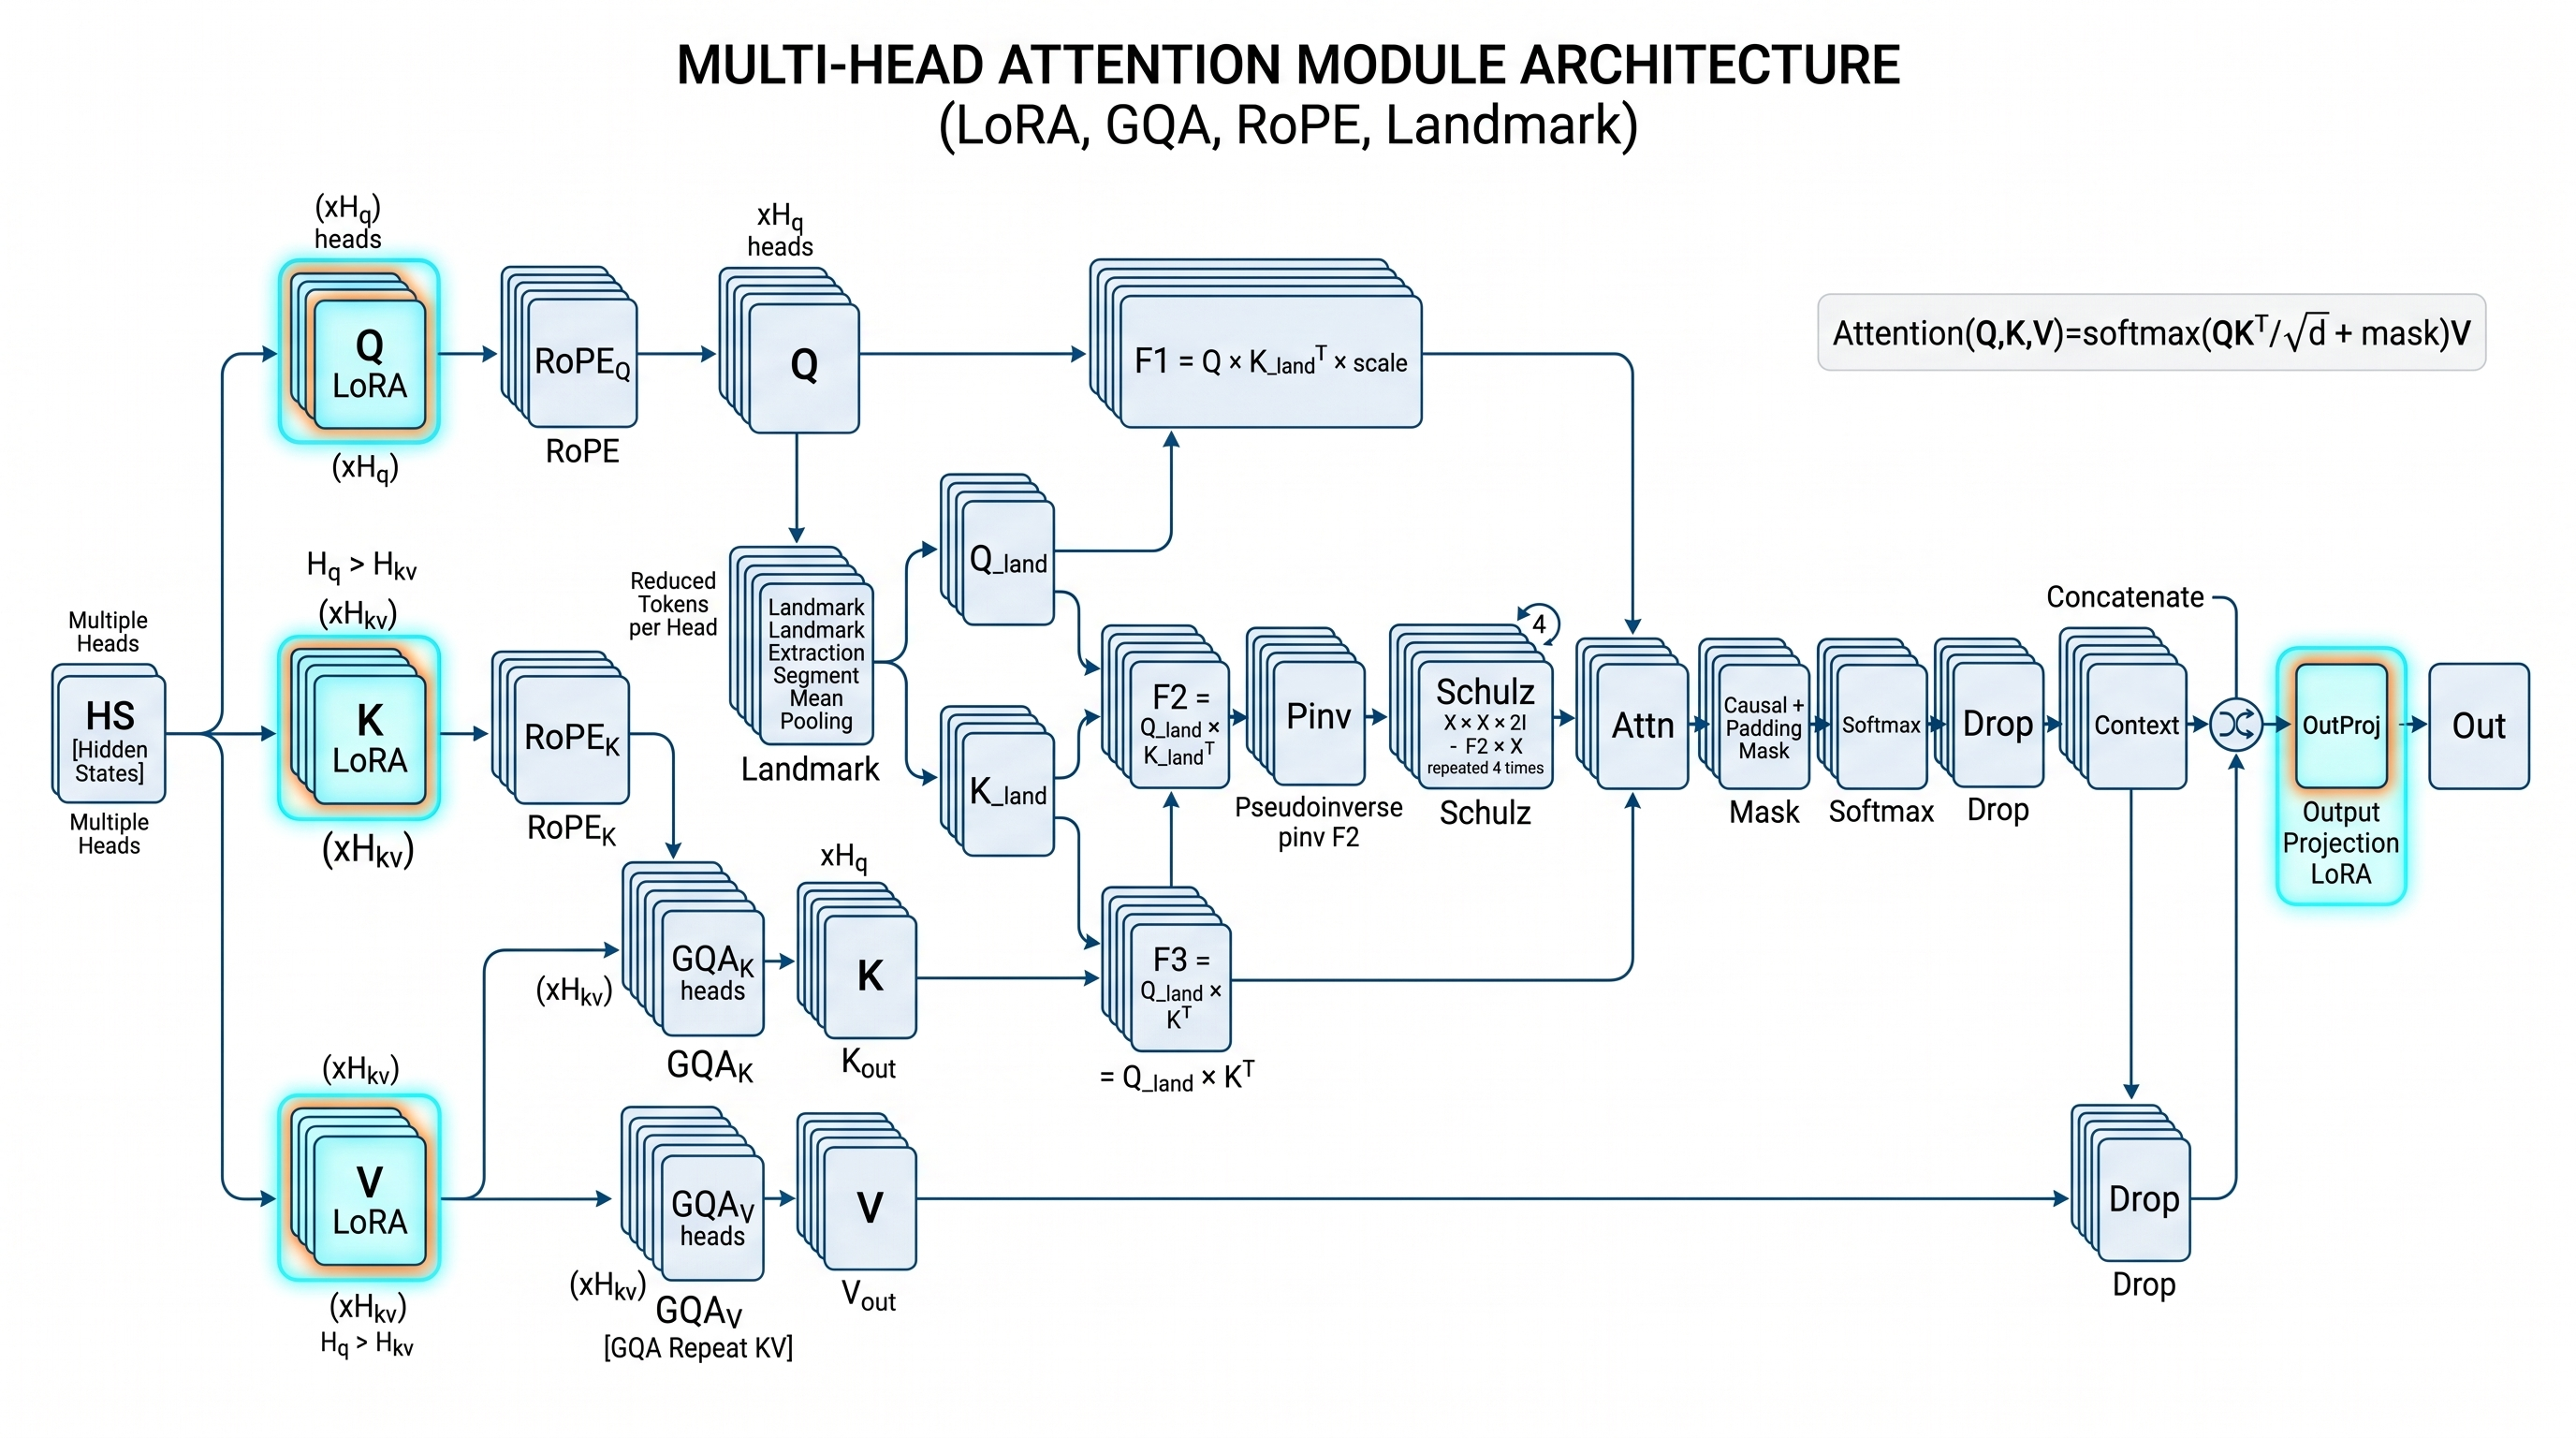
\includegraphics[width=\linewidth]{figures/architecture.jpeg}
\caption{High-level architectural diagram of nystrom\_attention.}
\label{fig:arch_nystrom-attention}
\end{figure}

